% arara: latex: { interaction: nonstopmode, options: ['-halt-on-error'] }
% arara: dvisvgm: { options: ['--no-fonts', '--exact-bbox', '--zoom=-1'] }
\documentclass[tikz,border=8pt,11pt]{standalone}
\usepackage{amsmath}
\definecolor{circleblue}{HTML}{0072B2}
\definecolor{pointred}{HTML}{D55E00}
\definecolor{fixedpurple}{HTML}{8B4C9D}
\definecolor{ink}{HTML}{25313C}
\definecolor{muted}{HTML}{7C8792}
\tikzset{point label/.style={inner sep=4pt,text=ink}}

\begin{document}
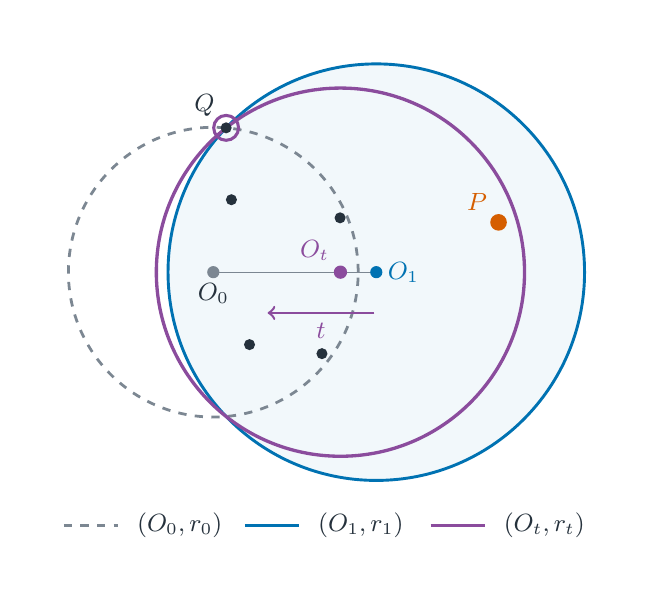
\begin{tikzpicture}[x=1.15cm,y=1.15cm,font=\small,text=ink]
  \fill[white] (-3.05,-3.25) rectangle (3.6,2.7);
  % Schematic for the contradictory assumption: P is inside (O_1,r_1).
  % O_0=(-1,0), r_0=1.6; O_1=(0.8,0), r_1=2.3; t=0.22.
  % O_t=(0.404,0); r_t^2=0.78*2.3^2+0.22*1.6^2-0.22*0.78*1.8^2.
  \draw[circleblue,fill=circleblue!5,line width=1.05pt]
    (0.8,0) circle[radius=2.3];
  \draw[muted,dashed,line width=1pt] (-1,0) circle[radius=1.6];
  \draw[fixedpurple,line width=1.2pt]
    (0.404,0) circle[radius={sqrt(4.133416)}];
  \draw[muted] (-1,0) -- (0.8,0);
  \draw[->,fixedpurple,line width=0.9pt] (0.78,-0.45) -- (-0.4,-0.45)
    node[midway,below] {$t$};
  \foreach \px/\py in {-0.8/0.8,-0.6/-0.8,0.2/-0.9,0.4/0.6}{
    \fill[ink] (\px,\py) circle[radius=2pt];
  }
  \fill[pointred] (2.15,0.55) circle[radius=3pt]
    node[point label,above left,text=pointred] {$P$};
  % A shared boundary point stays on every interpolated circle.
  \pgfmathsetmacro{\qx}{-1+0.51/3.6}
  \pgfmathsetmacro{\qy}{sqrt(1.6^2-(0.51/3.6)^2)}
  \fill[ink] (\qx,\qy) circle[radius=2pt];
  \draw[fixedpurple,line width=1.1pt] (\qx,\qy) circle[radius=4.5pt];
  \node[point label,above left] at (\qx,\qy) {$Q$};
  \fill[muted] (-1,0) circle[radius=2.2pt]
    node[point label,below] {$O_0$};
  \fill[circleblue] (0.8,0) circle[radius=2.2pt]
    node[point label,right,text=circleblue] {$O_1$};
  \fill[fixedpurple] (0.404,0) circle[radius=2.4pt]
    node[point label,above left,text=fixedpurple] {$O_t$};
  \draw[muted,dashed,line width=1pt] (-2.65,-2.8) -- (-2.05,-2.8);
  \node[anchor=west] at (-1.95,-2.8) {$(O_0,r_0)$};
  \draw[circleblue,line width=1.05pt] (-0.65,-2.8) -- (-0.05,-2.8);
  \node[anchor=west] at (0.05,-2.8) {$(O_1,r_1)$};
  \draw[fixedpurple,line width=1.2pt] (1.4,-2.8) -- (2,-2.8);
  \node[anchor=west] at (2.1,-2.8) {$(O_t,r_t)$};
\end{tikzpicture}
\end{document}
